% Options for packages loaded elsewhere
\PassOptionsToPackage{unicode}{hyperref}
\PassOptionsToPackage{hyphens}{url}
%
\documentclass[
]{article}
\usepackage{lmodern}
\usepackage{amssymb,amsmath}
\usepackage{ifxetex,ifluatex}
\ifnum 0\ifxetex 1\fi\ifluatex 1\fi=0 % if pdftex
  \usepackage[T1]{fontenc}
  \usepackage[utf8]{inputenc}
  \usepackage{textcomp} % provide euro and other symbols
\else % if luatex or xetex
  \usepackage{unicode-math}
  \defaultfontfeatures{Scale=MatchLowercase}
  \defaultfontfeatures[\rmfamily]{Ligatures=TeX,Scale=1}
\fi
% Use upquote if available, for straight quotes in verbatim environments
\IfFileExists{upquote.sty}{\usepackage{upquote}}{}
\IfFileExists{microtype.sty}{% use microtype if available
  \usepackage[]{microtype}
  \UseMicrotypeSet[protrusion]{basicmath} % disable protrusion for tt fonts
}{}
\makeatletter
\@ifundefined{KOMAClassName}{% if non-KOMA class
  \IfFileExists{parskip.sty}{%
    \usepackage{parskip}
  }{% else
    \setlength{\parindent}{0pt}
    \setlength{\parskip}{6pt plus 2pt minus 1pt}}
}{% if KOMA class
  \KOMAoptions{parskip=half}}
\makeatother
\usepackage{xcolor}
\IfFileExists{xurl.sty}{\usepackage{xurl}}{} % add URL line breaks if available
\IfFileExists{bookmark.sty}{\usepackage{bookmark}}{\usepackage{hyperref}}
\hypersetup{
  pdftitle={Intergenerational empowerment and early sexual onset among female adolescents: Evidence from a prevalence study in Ecuador},
  pdfauthor={Alonso Quijano},
  hidelinks,
  pdfcreator={LaTeX via pandoc}}
\urlstyle{same} % disable monospaced font for URLs
\usepackage[margin=1in]{geometry}
\usepackage{graphicx}
\makeatletter
\def\maxwidth{\ifdim\Gin@nat@width>\linewidth\linewidth\else\Gin@nat@width\fi}
\def\maxheight{\ifdim\Gin@nat@height>\textheight\textheight\else\Gin@nat@height\fi}
\makeatother
% Scale images if necessary, so that they will not overflow the page
% margins by default, and it is still possible to overwrite the defaults
% using explicit options in \includegraphics[width, height, ...]{}
\setkeys{Gin}{width=\maxwidth,height=\maxheight,keepaspectratio}
% Set default figure placement to htbp
\makeatletter
\def\fps@figure{htbp}
\makeatother
\setlength{\emergencystretch}{3em} % prevent overfull lines
\providecommand{\tightlist}{%
  \setlength{\itemsep}{0pt}\setlength{\parskip}{0pt}}
\setcounter{secnumdepth}{-\maxdimen} % remove section numbering
\usepackage{dcolumn}
\usepackage{booktabs}
\usepackage{longtable}
\usepackage{array}
\usepackage{multirow}
\usepackage{wrapfig}
\usepackage{float}
\usepackage{colortbl}
\usepackage{pdflscape}
\usepackage{tabu}
\usepackage{threeparttable}
\usepackage{threeparttablex}
\usepackage[normalem]{ulem}
\usepackage{makecell}
\usepackage{xcolor}
\newlength{\cslhangindent}
\setlength{\cslhangindent}{1.5em}
\newenvironment{cslreferences}%
  {\setlength{\parindent}{0pt}%
  \everypar{\setlength{\hangindent}{\cslhangindent}}\ignorespaces}%
  {\par}

\title{Intergenerational empowerment and early sexual onset among female
adolescents: Evidence from a prevalence study in Ecuador}
\author{Alonso Quijano}
\date{}

\begin{document}
\maketitle

The age of puberty onset has decreased substantially over the past
decades (Bellis, Downing, and Ashton 2006). Reasons exist to be
concerned about this fact as early sexual debut has been linked to
several adverse outcomes. Early sexual initiators have been found to be
more prone to having multiple sex partners, forcing partners to have
sex, having frequent sexual intercourse, and being engaged in teenage
pregnancy (O'Donnell, O'Donnell, and Stueve 2001). Studies performed on
different populations have also shown an association between early
initiation of sexual intercourse and HIV and other STDs risks
(e.g.~Kaestle et al. 2005; Stöckl et al. 2013). One major cause of the
high prevalence of STDs and unwanted pregnancies among young males and
females is that those who engage in early sexual activityare much less
likely to use contraception (Finer and Philbin 2013). Additionally, even
for those who manage to avoid pregnancy at first intercourse despite not
using contraception, chances of experiencing early childbearing remain
high since those who fail to use contraception at first sex are more
likely to continue engaging in risky sexual behavior in the future (St
Lawrence and Scott 1996; Magnusson, Masho, and Lapane 2012).

Many studies have tested the relationship between precocious sexual
initiation and household structure (e.g.~Ellis et al. 2003; Newcomer and
Udry 1987) and parental involvement (e.g.~Romer et al. 1999; Sieverding
et al. 2005; Velez-Pastrana, Gonzadez-Rodriguez, and Borges-Hernandez
2005). However, few studies have explored the intergenerational
transmission of behavioral patterns, such as how the timing of sexual
debut may be replicated across generations (e.g.~Johnson and Tyler
2007). This paper aims to examine the predicting ability of maternal
behavioral variables, including the mother's age at first intercourse,
and other mechanisms in which the mother's control of her sexual
decisions can be passed on to her daughter's own decision making. It is
plausible to believe that those mothers with low bargaining power may
directly or indirectly transmit their norms and beliefs to their
daughters, who may as well then become unable to exercise
decision-making over their sexuality. Parkes et al.~(2011) found that
talking about sex and contraception with children was negatively
correlated with delayed sexual initiation, suggesting that parents may
be able to shape their children's skills for negotiating sexual
situations. The influence intra-household sexual bargaining has on
children has yet been explored in experimental research. Therefore, this
study opens up an opportunity to discuss more in depth how sexual values
may be inherited and how they can relate to the sexual well-being of
young women.

\hypertarget{methods}{%
\subsection{METHODS}\label{methods}}

\hypertarget{data-and-sample}{%
\subsection{Data and sample}\label{data-and-sample}}

We used data from the 2018 National Health and Nutrition Survey of
Ecuador (Ensanut), which is conducted every five years by the National
Statistics Institute of Ecuador. Its goal is to assess the health and
nutritional status of adults and children in Ecuador. In 2018, the
survey gathered data from 43,311 households, totaling a number of
168,747 subjects. Measures of anthropometric, nutrition, economic status
were collected for all the members of the household. Data about the
sexual health of women was gathered for all those between 12 and 49
years old. Information about risk factors (e.g.~smoking and drinking)
was collected for only one random subject (male or female) between 5 and
18.

To perform the analysis, we selected the data of girls who were 16 years
old at the time of the interview and their mothers. Because the
independent variables we are interested in are the mothers' sexual
bargaining ability and age at first intercourse, we filtered those girls
who were currently living with their mothers and their mothers' partner
(which in most cases was the father). Additionally, since information
regarding sexuality was only gathered for women at age 49 or younger, we
only considered those whose mother was under that age threshold.
Finally, as data about drug use were not obtained for every subject (due
to the random selection), we decided to perform the analysis on two
samples: one larger sample that does not include these additional
confounders and a smaller one that includes them.

\hypertarget{measures}{%
\subsection{Measures}\label{measures}}

As in most studies that use secondary data, not all variables necessary
to understand the sexual activity of young females were available in
Ensanut. Nevertheless, we still were able to add several of the factors
that have been previously associated with early sexual debut.

The dependent variable for the analysis was \emph{early sexual
activity}. The 16-year-old girls who reported having had sexual
intercourse were coded as 1, whereas those who reported being virgin
were coded as 0. The 16-year-old cutoff has been used in previous
studies to demarcate early onset of sexual activity (e.g.~Ellis et al.
2003; Paul et al. 2000).

Basic sociodemographic and economic measures included ethnicity (whether
the girl identified herself as an ethnic minority), geographic area
(urban or rural), whether the girl was attending school, and household
income in US dollars. We used income as a measure of poverty. However,
evidence favors the use of consumption as a more effective tool to
measure well-being in developing countries (Meyer and Sullivan 2003).
Since consumption was not available in the survey, we added other
variables, including access to internet and the number of household
members. The number of household members was the most predicting factor
for impoverishment used in the Poverty Probability Index (Schreiner
2015).

Individual-level measures consisted of knowledge about sexuality and
risk behaviors. Sexuality knowledge was estimated through questions
about menstruation, pregnancy, and AIDs. Girls were asked whether they
knew what was happening to their body when they hay their first period,
whether a woman could become pregnant at first intercourse, and whether
HIV could spread through handshake. They were also asked whether they
had ever learned about sexual relationships, and if so, from whom they
had learned about (school, family, and others). Risk factors included
whether the girl had ever drunk alcohol or smoked in the past.

Mother-related variables included the mother's sexual bargaining
ability, age at first intercourse, and whether she had a teenage birth.
Mothers were asked if they could say no to their sexual partners
whenever they did not want to have sexual intercourse. For those who
were not using any form of contraception but would prefer to use one,
they were asked whether they thought their partner would be willing to
use it or not. Mothers who were unable to turn down sex or demand their
partner to use contraception were classified as low sexual bargaining.
We also considered variables such as occupation and education.

\hypertarget{results}{%
\subsection{RESULTS}\label{results}}

After cleaning up the data, the sample contained answers from 828
16-year-old girls and their respective mothers. Among those, 16.4\% had
ever had sexual intercourse, while 83.6\% had not. Table 1 shows the
percentage and mean levels of the explanatory variables by each group.
Mean differences of the categorical and continuous variables were tested
using the chi-square and t-test, respectively.

As seen in Table 1, across the two groups, girls who were sexually
active were more likely to belong to an ethnic minority (p \textless{}
.001), live in a rural area (p \textless{} .05), lack internet access (p
\textless{} .001), and miss school (p \textless{} .001). As for
sexuality knowledge, they tended to incorrectly answer the question
about AIDs (p \textless{} .05) and not know what was happening to their
body when they had their first period (p \textless{} .001). Sexually
active girls were more likely to learn about sexuality from family (p
\textless{} .05) and other sources (e.g., internet) (p \textless{}
.001). In contrast, non-sexually active girls were more prone to
learning from school (p \textless{} .001).

Mother characteristics significantly differed across groups. Mothers of
early sexual initiators were less likely to have finished high school (p
\textless{} .1) and more likely to have become a teenage parent (p
\textless{} .001). Mothers of early sexual initiators were also less
likely to be sexually empowered, although this difference was not shown
to be statistically significant.

\begin{table}

\caption{\label{tab:unnamed-chunk-1}Percentage and mean levels of explanatory variables by group}
\centering
\begin{threeparttable}
\begin{tabular}[t]{lrrl}
\toprule
Variables & Early sexual activity & No early sexual activity & p value\\
\midrule
Ethnic minority & 0.30 & 0.21 & 0.001 ***\\
Lives in a rural area & 0.48 & 0.41 & 0.033 *\\
Does not have internet & 0.75 & 0.55 & 0.000 ***\\
Misses school & 0.44 & 0.05 & 0.000 ***\\
Lacks knowledge about period & 0.28 & 0.19 & 0.000 ***\\
\addlinespace
Lacks knowledge about pregnancy & 0.20 & 0.17 & 0.273\\
Lacks knowledge about AIDs & 0.18 & 0.12 & 0.014 *\\
Does not know about sexuality & 0.09 & 0.07 & 0.273\\
Knows about sexuality from family & 0.15 & 0.10 & 0.015 *\\
Knows about sexuality from school & 0.68 & 0.80 & 0.000 ***\\
\addlinespace
Knows about sexuality from other sources & 0.08 & 0.03 & 0.000 ***\\
Has ever drunk alcohol & 0.62 & 0.44 & 0.000 ***\\
Has ever smoked & 0.09 & 0.03 & 0.000 ***\\
Mother has a job & 0.64 & 0.60 & 0.282\\
Mother finished HS & 0.44 & 0.51 & 0.1  .\\
\addlinespace
Mother had a teenage birth & 0.68 & 0.48 & 0.000 ***\\
Mother lacks sexual bargaining & 0.15 & 0.11 & 0.108\\
Household income & 646.79 & 630.03 & 0.944\\
Number of members in the household & 5.64 & 5.42 & 0.08  .\\
Mother's age at first intercourse & 16.11 & 17.64 & 0.000 ***\\
\bottomrule
\end{tabular}
\begin{tablenotes}[para]
\item \textit{Note: } 
\item p values for comparison of percentagges using chi-square. p values for comparison of means using t-test. Ns = 401–828. . < .1. *p < .05. **p < .01. ***p < .001.
\end{tablenotes}
\end{threeparttable}
\end{table}

As expected, early sexual initiators were more likely to have been
reared by a mother who had herself had her first coitus at a very young
age. Figure 1 illustrates the cumulative histogram of age at first
coitus of the mothers. The figure clearly shows that mothers of early
sexual initiators had their first coitus at a younger age than mothers
of those who were not sexually active. The mean age of first coitus for
each group was 16.11 (SD = 2.48) and 17.76 (SD = 2.79), respectively.
The t-test showed that these differences were unlikely to have been due
to chance (p \textless{} .001).

\begin{figure}

{\centering 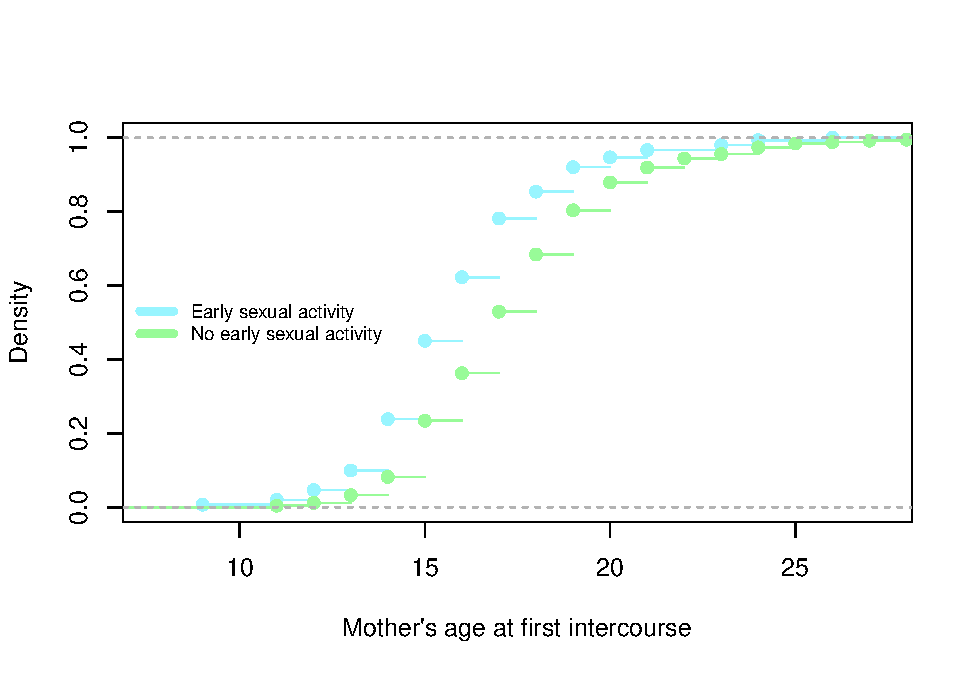
\includegraphics[width=0.8\linewidth,height=0.7\textheight]{early_sexual_activity_report_files/figure-latex/unnamed-chunk-2-1} 

}

\caption{Cumulative histogram of age at first intercourse of mothers by group}\label{fig:unnamed-chunk-2}
\end{figure}

\begin{table}[!htbp] \centering 
  \caption{Logistic Regression Results} 
  \label{} 
\begin{tabular}{@{\extracolsep{5pt}}lD{.}{.}{-3} D{.}{.}{-3} } 
\\[-1.8ex]\hline 
\hline \\[-1.8ex] 
 & \multicolumn{2}{c}{\textit{Dependent variable:}} \\ 
\cline{2-3} 
\\[-1.8ex] & \multicolumn{2}{c}{early\_sexual\_activity} \\ 
\\[-1.8ex] & \multicolumn{1}{c}{(1)} & \multicolumn{1}{c}{(2)}\\ 
\hline \\[-1.8ex] 
 ruralyes & -0.077 & -0.056 \\ 
  & (0.231) & (0.232) \\ 
  & & \\ 
 h\_income & 0.0001 & 0.0001 \\ 
  & (0.0001) & (0.0001) \\ 
  & & \\ 
 h\_num\_members & 0.097^{*} & 0.068 \\ 
  & (0.056) & (0.057) \\ 
  & & \\ 
 h\_internetno & 0.481^{**} & 0.485^{**} \\ 
  & (0.241) & (0.244) \\ 
  & & \\ 
 minorityyes & 0.349 & 0.356 \\ 
  & (0.254) & (0.257) \\ 
  & & \\ 
 attends\_schoolno & 2.151^{***} & 2.164^{***} \\ 
  & (0.317) & (0.321) \\ 
  & & \\ 
 period\_knowledgeno & 0.257 & 0.243 \\ 
  & (0.251) & (0.252) \\ 
  & & \\ 
 aids\_knowledgeno & 0.004 & 0.072 \\ 
  & (0.307) & (0.308) \\ 
  & & \\ 
 pregnancy\_knowledgeno & 0.289 & 0.321 \\ 
  & (0.259) & (0.260) \\ 
  & & \\ 
 sexuality\_knowledgefamily & 2.394^{**} & 2.252^{**} \\ 
  & (1.081) & (1.097) \\ 
  & & \\ 
 sexuality\_knowledgeschool & 1.841^{*} & 1.809^{*} \\ 
  & (1.050) & (1.065) \\ 
  & & \\ 
 sexuality\_knowledgeother & 2.821^{**} & 2.714^{**} \\ 
  & (1.135) & (1.150) \\ 
  & & \\ 
 m\_jobyes & 0.613^{***} & 0.563^{**} \\ 
  & (0.224) & (0.226) \\ 
  & & \\ 
 m\_finished\_HSyes & 0.393^{*} & 0.449^{**} \\ 
  & (0.227) & (0.228) \\ 
  & & \\ 
 m\_empowermentno & 0.633^{**} & 0.595^{**} \\ 
  & (0.295) & (0.298) \\ 
  & & \\ 
 m\_teenage\_birthyes &  & 0.767^{***} \\ 
  &  & (0.218) \\ 
  & & \\ 
 Constant & -5.525^{***} & -5.802^{***} \\ 
  & (1.150) & (1.170) \\ 
  & & \\ 
\hline \\[-1.8ex] 
Observations & \multicolumn{1}{c}{828} & \multicolumn{1}{c}{824} \\ 
Log Likelihood & \multicolumn{1}{c}{-323.140} & \multicolumn{1}{c}{-316.344} \\ 
Akaike Inf. Crit. & \multicolumn{1}{c}{678.279} & \multicolumn{1}{c}{666.689} \\ 
\hline 
\hline \\[-1.8ex] 
\textit{Note:}  & \multicolumn{2}{r}{$^{*}$p$<$0.1; $^{**}$p$<$0.05; $^{***}$p$<$0.01} \\ 
\end{tabular} 
\end{table}

\hypertarget{references}{%
\subsection*{References}\label{references}}
\addcontentsline{toc}{subsection}{References}

\hypertarget{refs}{}
\begin{cslreferences}
\leavevmode\hypertarget{ref-bellis2006adults}{}%
Bellis, Mark A, J Downing, and JR Ashton. 2006. ``Adults at 12? Trends
in Puberty and Their Public Health Consequences.'' BMJ Publishing Group
Ltd.

\leavevmode\hypertarget{ref-ellis2003does}{}%
Ellis, Bruce J, John E Bates, Kenneth A Dodge, David M Fergusson, L John
Horwood, Gregory S Pettit, and Lianne Woodward. 2003. ``Does Father
Absence Place Daughters at Special Risk for Early Sexual Activity and
Teenage Pregnancy?'' \emph{Child Development} 74 (3): 801--21.

\leavevmode\hypertarget{ref-finer2013sexual}{}%
Finer, Lawrence B, and Jesse M Philbin. 2013. ``Sexual Initiation,
Contraceptive Use, and Pregnancy Among Young Adolescents.''
\emph{Pediatrics} 131 (5): 886--91.

\leavevmode\hypertarget{ref-johnson2007adolescent}{}%
Johnson, Katherine A, and Kimberly A Tyler. 2007. ``Adolescent Sexual
Onset: An Intergenerational Analysis.'' \emph{Journal of Youth and
Adolescence} 36 (7): 939--49.

\leavevmode\hypertarget{ref-kaestle2005young}{}%
Kaestle, Christine E, Carolyn T Halpern, William C Miller, and Carol A
Ford. 2005. ``Young Age at First Sexual Intercourse and Sexually
Transmitted Infections in Adolescents and Young Adults.'' \emph{American
Journal of Epidemiology} 161 (8): 774--80.

\leavevmode\hypertarget{ref-magnusson2012early}{}%
Magnusson, Brianna M, Saba W Masho, and Kate L Lapane. 2012. ``Early Age
at First Intercourse and Subsequent Gaps in Contraceptive Use.''
\emph{Journal of Women's Health} 21 (1): 73--79.

\leavevmode\hypertarget{ref-meyer2003measuring}{}%
Meyer, Bruce D, and James X Sullivan. 2003. ``Measuring the Well-Being
of the Poor Using Income and Consumption.'' National Bureau of Economic
Research.

\leavevmode\hypertarget{ref-newcomer1987parental}{}%
Newcomer, Susan, and J Richard Udry. 1987. ``Parental Marital Status
Effects on Adolescent Sexual Behavior.'' \emph{Journal of Marriage and
the Family}, 235--40.

\leavevmode\hypertarget{ref-o2001early}{}%
O'Donnell, Lydia, Carl R O'Donnell, and Ann Stueve. 2001. ``Early Sexual
Initiation and Subsequent Sex-Related Risks Among Urban Minority Youth:
The Reach for Health Study.'' \emph{Family Planning Perspectives},
268--75.

\leavevmode\hypertarget{ref-parkes2011parenting}{}%
Parkes, Alison, Marion Henderson, Daniel Wight, and Catherine Nixon.
2011. ``Is Parenting Associated with Teenagers' Early Sexual
Risk-Taking, Autonomy and Relationship with Sexual Partners?''
\emph{Perspectives on Sexual and Reproductive Health} 43 (1): 30--40.

\leavevmode\hypertarget{ref-paul2000determinants}{}%
Paul, Charlotte, Julie Fitzjohn, Peter Herbison, and Nigel Dickson.
2000. ``The Determinants of Sexual Intercourse Before Age 16.''
\emph{Journal of Adolescent Health} 27 (2): 136--47.

\leavevmode\hypertarget{ref-romer1999parental}{}%
Romer, Daniel, Bonita Stanton, Jennifer Galbraith, Susan Feigelman,
Maureen M Black, and Xiaoming Li. 1999. ``Parental Influence on
Adolescent Sexual Behavior in High-Poverty Settings.'' \emph{Archives of
Pediatrics \& Adolescent Medicine} 153 (10): 1055--62.

\leavevmode\hypertarget{ref-schreiner2015ecuador}{}%
Schreiner, Mark. 2015. ``Ecuador 2013 Poverty Probability Index(PPI):
Design Memo.''

\leavevmode\hypertarget{ref-sieverding2005influence}{}%
Sieverding, John A, Nancy Adler, Stephanie Witt, and Jonathan Ellen.
2005. ``The Influence of Parental Monitoring on Adolescent Sexual
Initiation.'' \emph{Archives of Pediatrics \& Adolescent Medicine} 159
(8): 724--29.

\leavevmode\hypertarget{ref-st1996examination}{}%
St Lawrence, Janet S, and Catina P Scott. 1996. ``Examination of the
Relationship Between African American Adolescents' Condom Use at Sexual
Onset and Later Sexual Behavior: Implications for Condom Distribution
Programs.'' \emph{AIDS Education and Prevention}.

\leavevmode\hypertarget{ref-stockl2013early}{}%
Stöckl, Heidi, Naira Kalra, Jantine Jacobi, and Charlotte Watts. 2013.
``Is Early Sexual Debut a Risk Factor for Hiv Infection Among Women in
Sub-Saharan Africa? A Systematic Review.'' \emph{American Journal of
Reproductive Immunology} 69: 27--40.

\leavevmode\hypertarget{ref-velez2005family}{}%
Velez-Pastrana, Maria C, Rafael A Gonzadez-Rodriguez, and Adalisse
Borges-Hernandez. 2005. ``Family Functioning and Early Onset of Sexual
Intercourse in Latino Adolescents.'' \emph{Adolescence} 40 (160).
\end{cslreferences}

\end{document}
